
%---------------------------------------------
%	6. Application & Perform of GNN Algorithm
%---------------------------------------------

%\chapter{Application and Performance of GNN Algorithm}\label{chapter-6}

%The main application of the GNN algorithm on the trackML data, the data preparation, what data was exactly used and why, the ML classification algorithm used to build the edge connections. The main results we get from application of this algorithm, the track reconstruction efficiency, the purity metrics, computational performance. Comparison with other algorithms.

%nips-2018-competation
%Data.
%We used the fast (10s per event) and accurate simulation engine ACTS4 [6] to generate the challenge data. It allowed us to generate realistic data emulating a full Silicon LHC detector (see Fig 3), while providing us with the ground truth of particle trajectory membership. Thus, for each event we obtained the “detected” 3D points coordinates (and additional features), and, as ground truth, the list of points associated to each track. There is a one to one relationship between the true 3D points and the reconstructed ones.


\chapter{Application of the GNN Algorithm on the TrackML Model}
\label{chapter-6}

% This chapter focuses on the track finding algorithm development and its application on the publicly available dataset designed for the Kaggle TrackML challenge. The preliminary results related to track reconstruction efficiency and purity metrics are presented and discussed.

%The main application of the GNN algorithm on the trackML data, the data preparation, what data was exactly used and why, the ML classification algorithm used to build the edge connections. The main results we get from application of this algorithm, the track reconstruction efficiency, the purity metrics, computational performance. Comparison with other algorithms.


\section{Implementation}


\subsection{Data Preparation}
%Talk specifically about the TrackML data here and how it was prepared. How the trackml hits are converted into nodes and edges. Close proximity node merging. Checks that are put in place in order to make sure there are no hits that have the same module id (more than 2 hits that are simultaneously in the same module and volume and layer).



\subsection{Constructing Track State Estimates}
\label{constructing-track-states}

Track parameters in both the transverse $x$-$y$ plane and the $r$-$z$ plane are considered in order to construct track state estimates $X_{ij}$.


\subsubsection{Parabolic Model}
\label{parabolic-state}

In the $x$-$y$ plane, charged particles experience the influence of the magnetic field, so naturally their trajectories follow a near-parabolic shape. For a given node A, a parabola is formed using the origin O, node A and neighbour node B, illustrated in Figure \ref{fig:gnn-parabolic-model}. The parabola is transformed into the local coordinate system of node A such that the new $x$-axis, $X_A$ goes through the global origin O and node A. The parabolic parameters \{$a, b, c$\} are computed using equations Eq \eqref{eqn:parabolic-equations}. The measurement vector $[m_O \quad m_A \quad m_C]$ is obtained in the coordinate system local to node A, assuming $m_O = 0$ and $m_A = 0$.

\begin{equation}
\begin{aligned}
m_O = ax_{O}^{2} + bx_O + c \\
m_A = c \\
m_B = ax_{B}^{2} + bx_B + c
\end{aligned}
\label{eqn:parabolic-equations}
\end{equation}

\begin{figure}[htbp!] 
    \centering
    \subfloat[]{%
        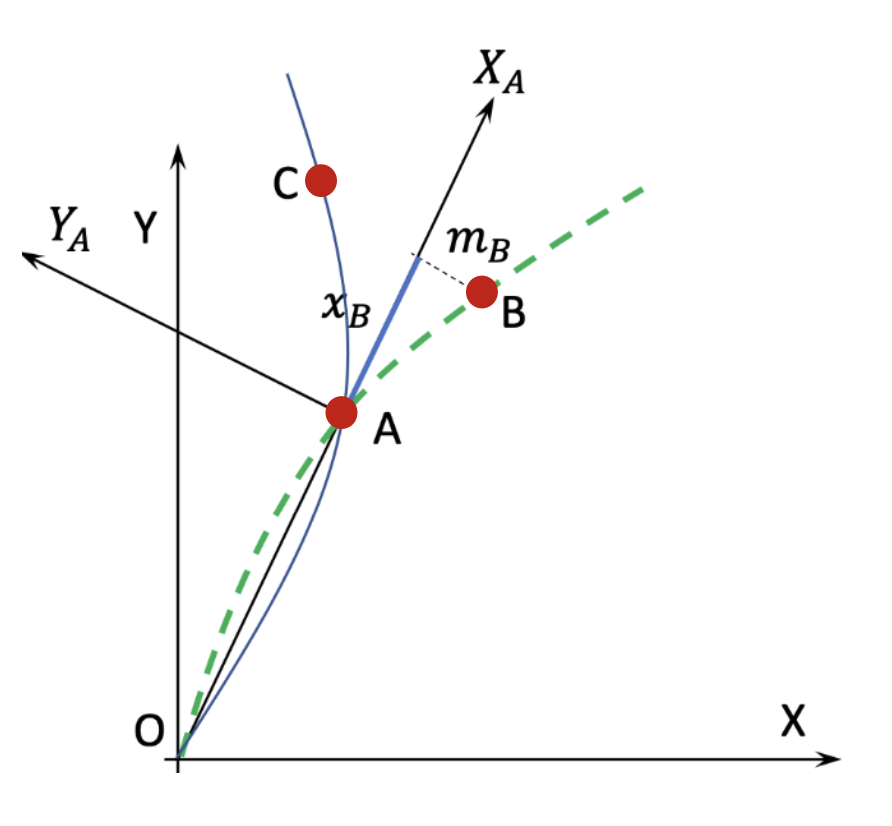
\includegraphics[width=0.43\textwidth]{images/5-gnn-algorithm/parabolic-state-model-1.png}%
        \label{fig:gnn-parabolic-state-1}%
        }%
    \hfill%
    \subfloat[]{%
        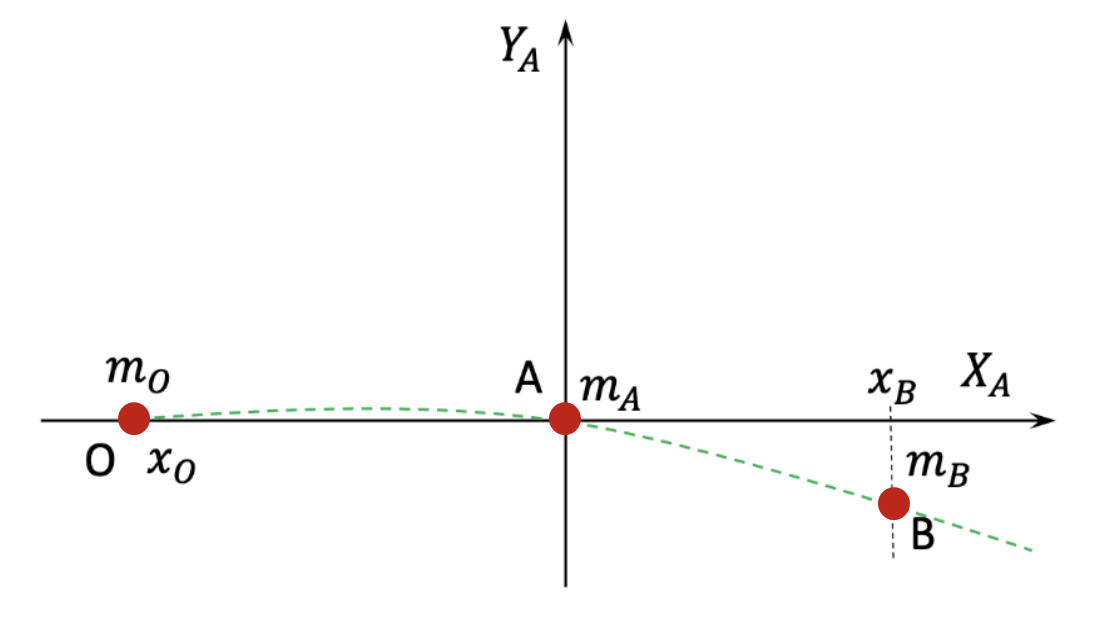
\includegraphics[width=0.57\textwidth]{images/5-gnn-algorithm/parabolic-state-model-2.png}%
        \label{fig:gnn-parabolic-state-2}%
        }%
    \caption{Illustrations of the parabolic model used in the $x$-$y$ plane. a) shows the construction of a parabola between the global origin, O and nodes A - B, as well as a second parabola between O - A - C. b) shows the rotation of the parabola O - A - B into the local coordinate system of node A.}
    \label{fig:gnn-parabolic-model}
\end{figure}


\subsubsection{Linear Model}
\label{linear-state}

The $r$-$z$ plane is parallel to the direction of travel of the beamline, where tracks follow a linear model. The inverse track inclination between a node and its neighbour, $\tau$, is used and is given by Eq \eqref{eqn:tau-parameter}, where $z_A$, $r_A$ refer to measurements of the node and $z_B$, $r_B$ refer to measurements of its neighbour. $r$ is the square root of the sum in quadrature of the $x$ and $y$ measurements.

\begin{equation}
\tau = \frac{z_A - z_B}{r_A - r_B}
\label{eqn:tau-parameter}
\end{equation}

\subsubsection{Track State Estimate}

Parabolic parameters $a$ and $b$ in the $x$-$y$ plane, as well as inverse track inclination $\tau$ in the $r$-$z$ plane give an indication of track orientation. For node $i$ and its neighbour $j$, the track state estimate $X_{ij}$ is given by Eq \eqref{eqn:joint-state-vector}

\begin{equation}
X_{ij} = \begin{bmatrix} a \\ b \\ \tau \end{bmatrix}
\label{eqn:joint-state-vector}
\end{equation}






\subsection{Derivation of Covariance}

\subsection{Moliere Theory of Multiple Scattering}
\begin{itemize}
\item highland formula and handling the error/effects due to multiple scattering for the barrel and endcap in slightly different ways
\item how were the covariances dervied and the sigma errors chosen
\item Derivation of the edge state covariance
\item 2 different ones, we start with the edge covariance, and derive the state covariance
\end{itemize}
% moliere theory links:
%https://gray.mgh.harvard.edu/attachments/article/337/Techniques%20of%20Proton%20Radiotherapy%20(06)%20Multiple%20Scattering.pdf
%https://pdg.lbl.gov/2005/reviews/passagerpp.pdf





\subsection{Determining the Optimal KL Threshold}
\label{chapter-6-kl-threshold}

If $d_{KL}$ $\leq$ some threshold, then states can be clustered together and merged into a single state.

To determine the optimal pairwise $d_{KL}$ between track state estimates $X_{ij}$ for a given node, a SVM classifier was trained using pairwise $d_{KL}$ and $\sigma_{e}$ as input features. A MC simulation of $10,000$ particle collision events, each event with ten truth tracks, was used to build a training dataset. Loosely compatible edge connections were formed using a hit-pair predictor based on track inclination angle of neighbouring hits. The feature vector was comprised of $\sigma_{e}$ for a given node, and pairwise $d_{KL}$ between track states. The ground truth particle was extracted for each pairwise connection, where truth 1 corresponded to hits from both track states originating from the same truth particle, and truth 0 otherwise. A SVM was trained to discriminate between the two classes \cite{scikit-learn}, using a polynomial degree three kernel. Predictions were adjusted such that the TPR was tuned to 95\% and the decision boundary was converted into a fast LUT using a similar methodology outlined in Section \ref{LUT-generation}.  Other classification algorithms were explored, however the SVM was the most appropriate in this instance to determine a decision boundary to best separate the classes.

\begin{figure}[htbp!] 
    \centering
    \subfloat[]{%
        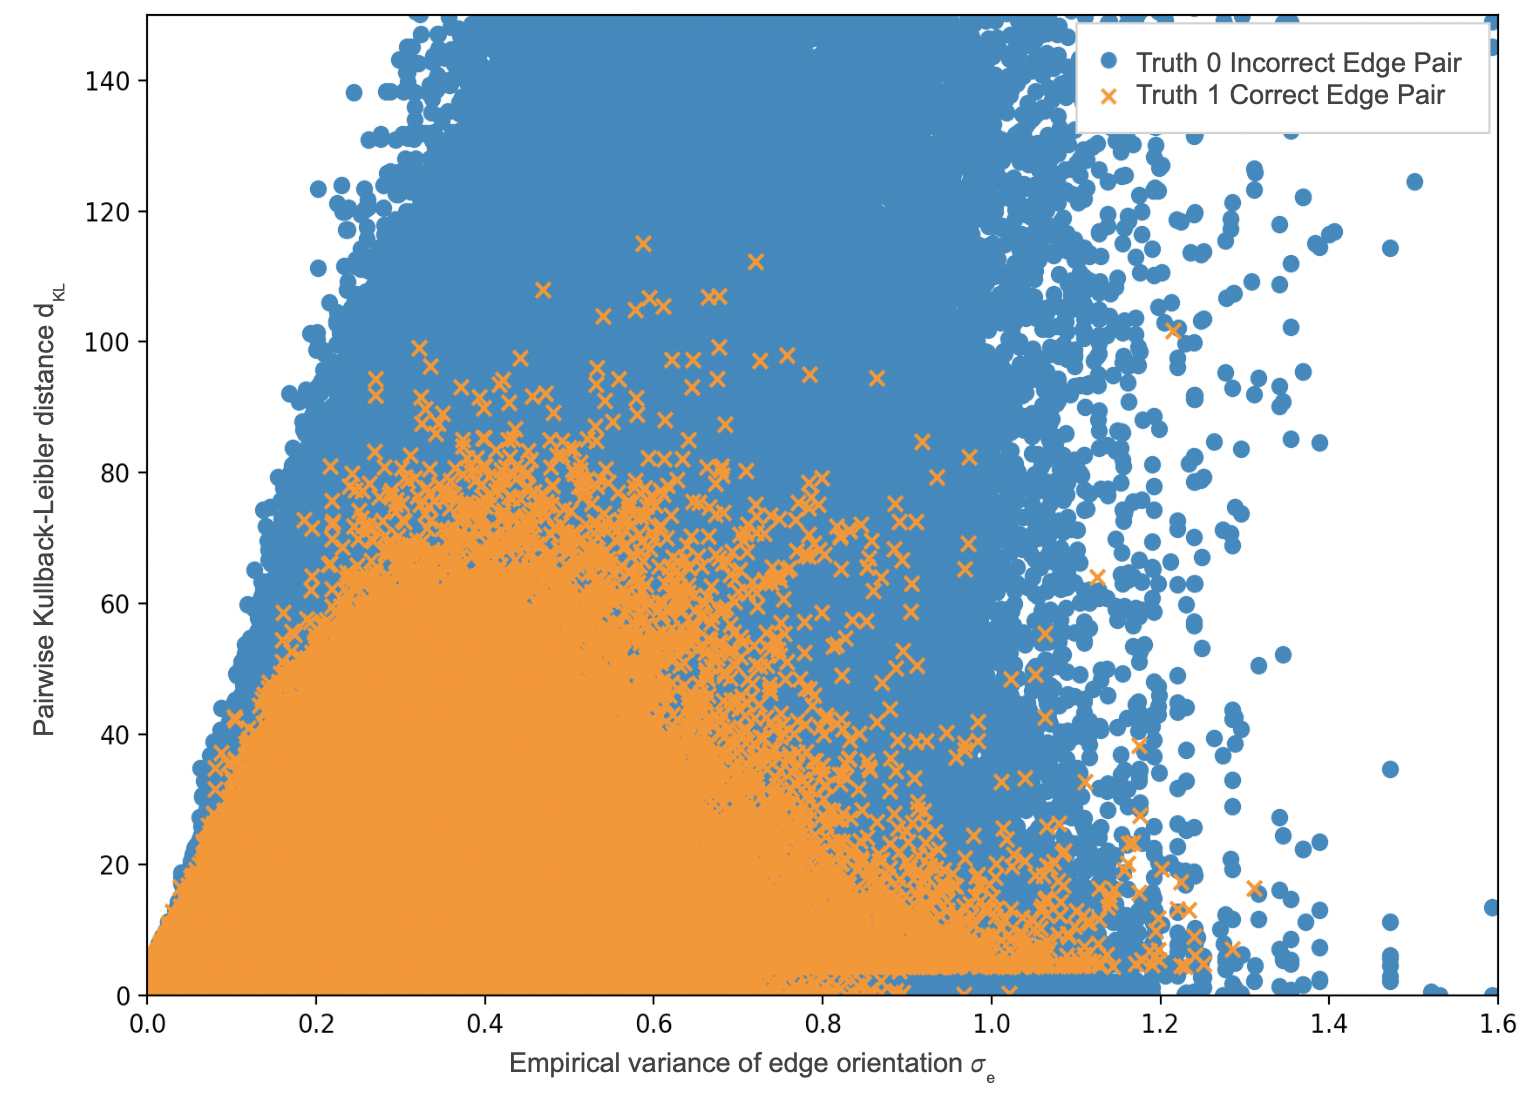
\includegraphics[width=0.8\linewidth]{images/6-results/kl-truth.png}%
        \label{fig:KL-distance-truth}%
        }%
    \hfill%
    \subfloat[]{%
        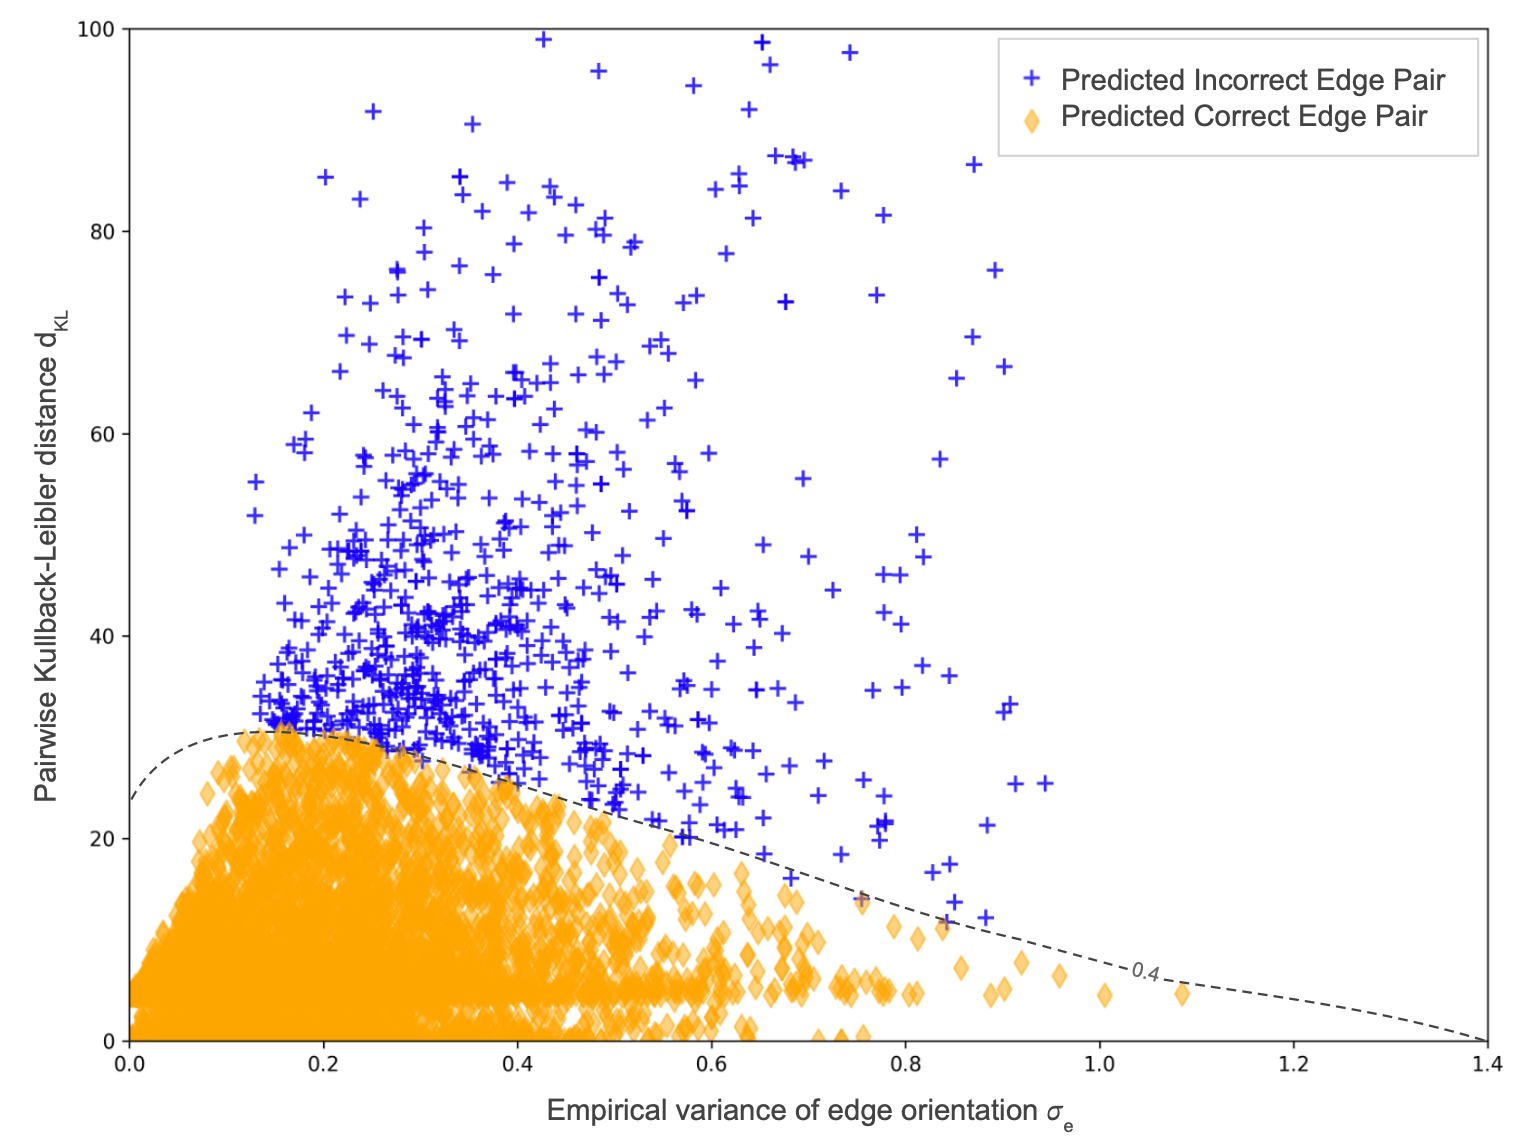
\includegraphics[width=0.8\linewidth]{images/6-results/kl-predictions.png}%
        \label{fig:KL-distance-predictions}%
        }%
    \caption{}
    \label{fig:KL-distance}
\end{figure}





\subsection{Extrapolation Models}
\label{chapter-6-extrapolation}
\subsubsection{Linear Extrapolation Model}
\subsubsection{Parabolic Extrapolation Model}
\begin{itemize}
    \item Information propagation via Message Passing Mechanism
    \item Extrapolation and Validation
    \item Linear and Parabolic model - 2 different extrapolations for xy componenets of state vector and rz componenet, illustrations here
    \item Kalman Filter Update, OU process for correlated noise
\end{itemize}

Mention here that both the linear and parabolic models were used in this instance, where the track state estimate comprised of a 3x1 vector, a, b, tau. The extrapolation and KF update will be different here, different transition Jacobian matrix. Also mention about tuning the chi2 distance thresholds during extrapolation

%The matrix $\widetilde{C}_{ij}$ includes the addition of the process noise $Q$ modelled by the Ornstein-Uhlenbeck (OU) process \cite{OU} which encompasses all material effects. See Section \ref{kf} for further details. The full derivation of $F$ and $Q$ are shown in Appendix \ref{appendix:Appendix-A}


\subsection{Implementation of Kalman Filters}
\label{gnn-kf-implementation}
Mention about the OU process noise, for correlated noise etc

%\begin{itemize}
%\item emphasis on the use of KFs both in information aggregation stage and in track extraction, both are implemented in different ways, is a useful and unique part to this algorithm
%\item OU process noise
%\end{itemize}



\section{Endcap Results and Performance Evaluation}

% track purity, particle purity, track reconstruction efficiency
% TODO: mention here that the parabolic track state model was used and the joint track state was used, and mention the section here

%nips-2018-competation
%Data.
%We used the fast (10s per event) and accurate simulation engine ACTS4 [6] to generate the challenge data. It allowed us to generate realistic data emulating a full Silicon LHC detector (see Fig 3), while providing us with the ground truth of particle trajectory membership. Thus, for each event we obtained the “detected” 3D points coordinates (and additional features), and, as ground truth, the list of points associated to each track. There is a one to one relationship between the true 3D points and the reconstructed ones.

%\begin{itemize}
%    \item Application on TrackML model, endcap volume only, metrics, performance eval etc, track reconstruction efficiency, track purity and particle purity, comparison with TrackML solutions
%    \item Track reconstruction efficiency, track purity, particle purity
%    \item Performance Evaluation
%    \item execution time?
%\end{itemize}


\section{Outlook}
\subsection{Extension to the Barrel Region}
\subsection{Software Optimisations}

\subsection{Other Approaches}
\subsubsection{Community Detection}
\subsubsection{Cellular Automatons}

%If a subgraph does not meet the criteria to qualify as a good track candidate, a \textit{Community Detection} algorithm \cite{community} is applied in order to further partition the set of nodes. Community Detection is a generalisation of CCA and works by using a distance metric, typically modularity, in order to label nodes as \textit{closely connected}. Modularity is a benefit function that measures the strength of a particular division of a network using the number of edges. A popular modularity maximisation approach is the Louvain method \cite{python_louvain}, which iteratively optimises local communities until global modularity can no longer be improved. An example illustration of a network partition via Community Detection is shown in Figure \ref{fig:community-detection}. Any subgraphs with zero extracted candidates through this procedure are propagated to further stages for additional processing.

%Community Detection: divides nodes into various clusters based on edge structure. It learns from edge weights, and distance and graph objects similarly. 

%\begin{figure}[htbp]
%    \centering
%    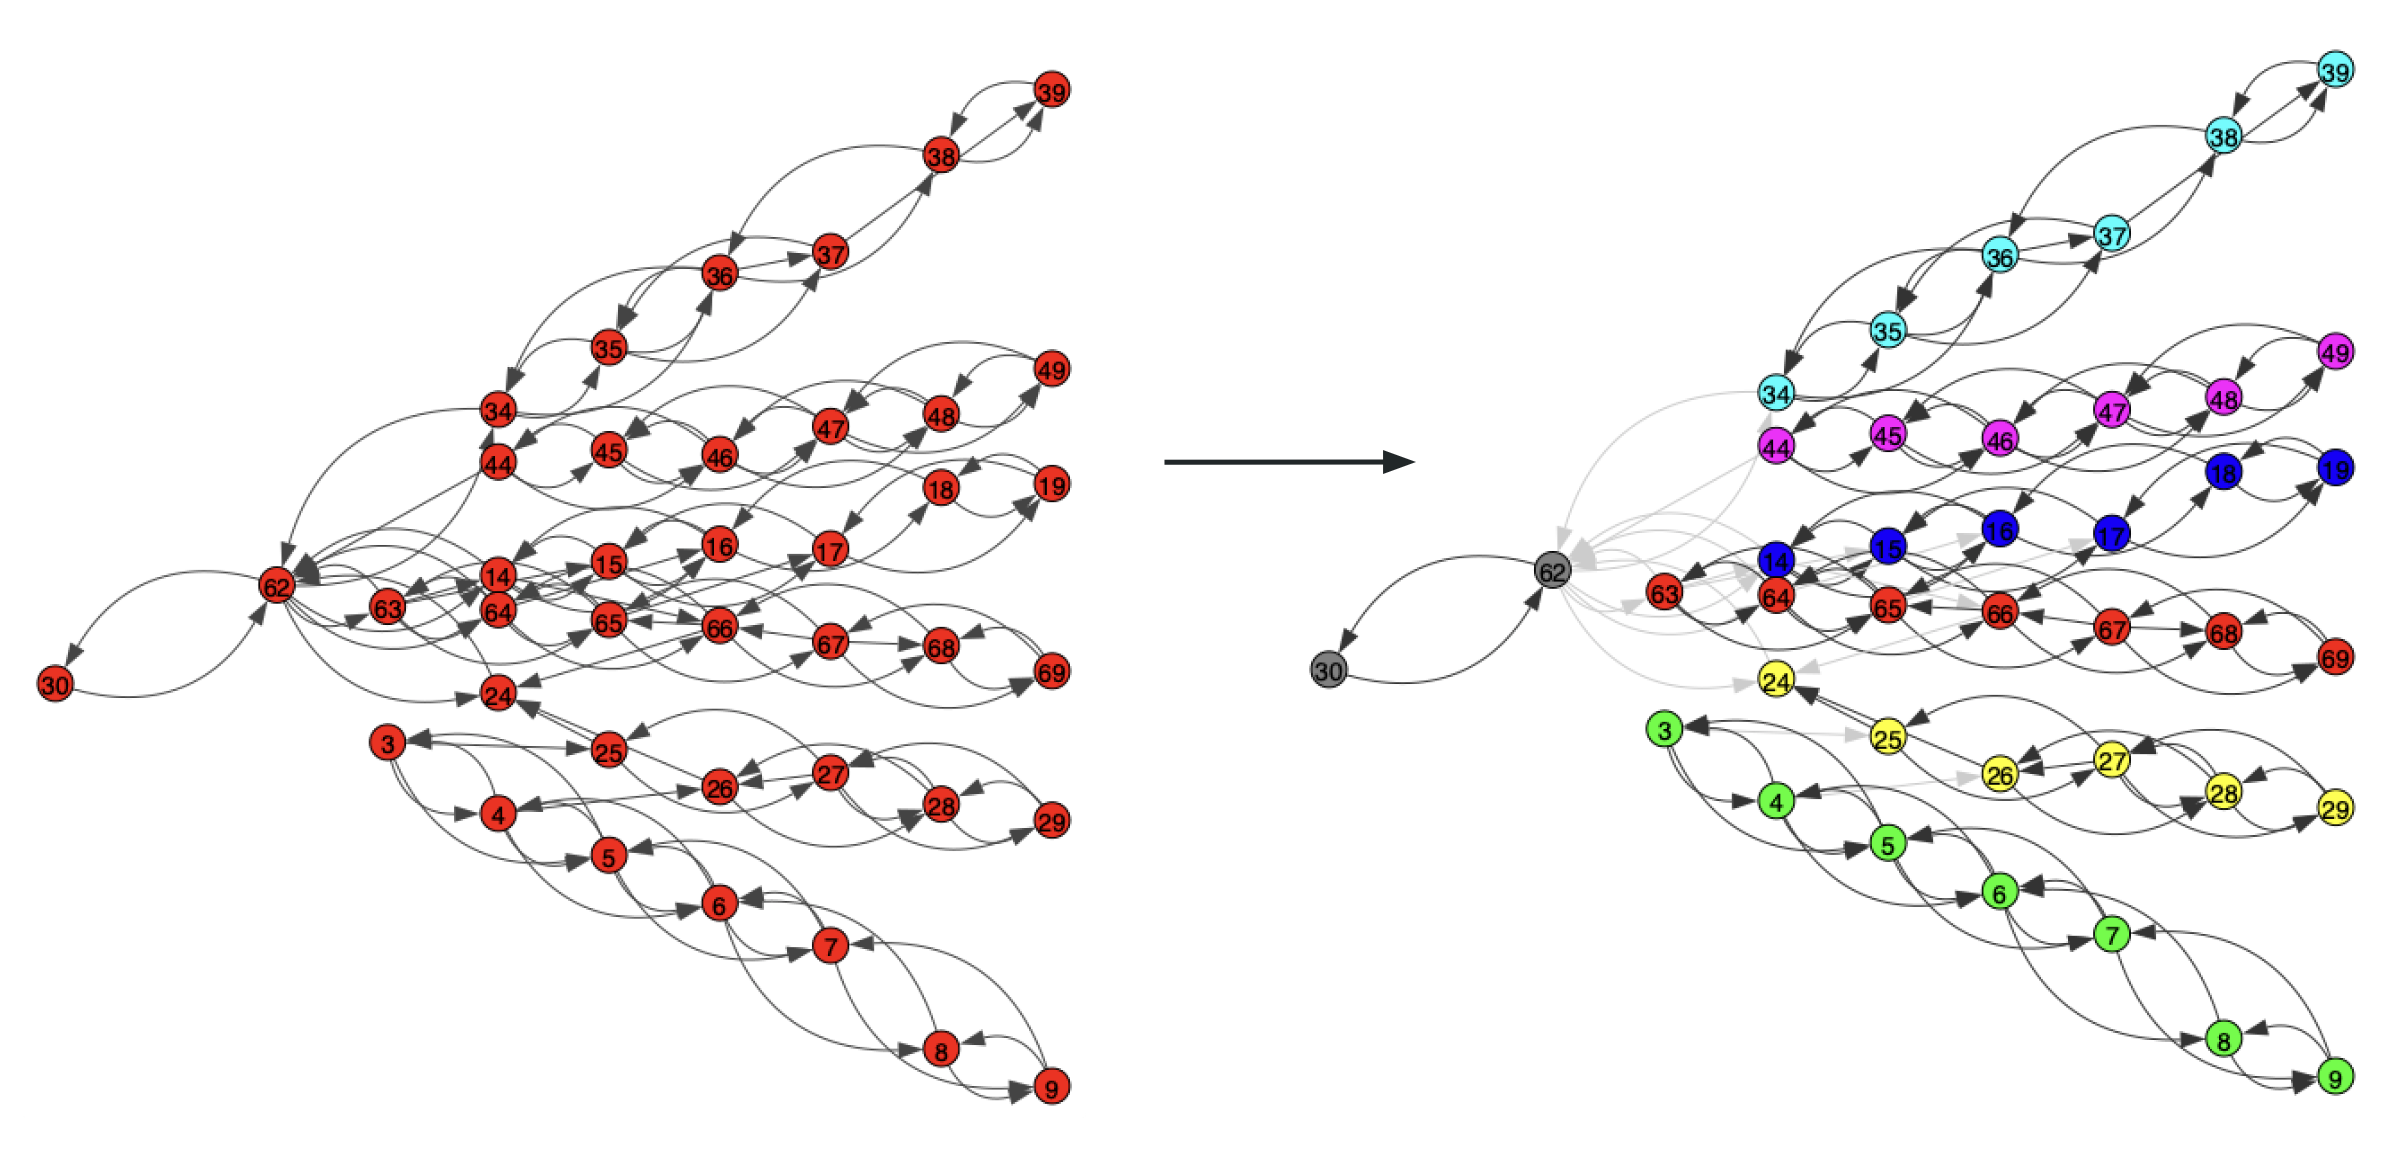
\includegraphics[width=0.98\textwidth]{images/5-gnn-algorithm/community-detection.png}
%    \caption{TODO: caption ....}
%    \label{fig:community-detection}%
%\end{figure}

%\begin{itemize}
%    \item extension to barrel, analysis of results, performance  evaluation, challenges and outlook
%    \item Optimisation - GPU acceleration etc
%\end{itemize}


\section{Conclusions}